% Use a one-sided article template
\documentclass[oneside,10pt]{article}
% Decrease the margins a little
\usepackage{fullpage}

% Support UTF8 input
\usepackage[utf8]{inputenc}

% Set up for including graphics
% We'll use png or pdf graphics
\usepackage[pdftex]{graphicx}
\DeclareGraphicsExtensions{.png,.pdf}

% Hyperref adds hyperlinks to the document automatically
% It's not much use yet, but it will be
\usepackage{hyperref}

% For including code into the document
\usepackage{verbatim}

% Tweak the default fonts a little
\renewcommand\rmdefault{bch}
\usepackage[small]{caption}
\usepackage[small]{titlesec}
\linespread{1.07}

% Typographic tweaks
\usepackage{microtype}
%\usepackage{}

\title{The Grammar of Graphics}
\author{Pedro Alcocer}
\date{\today}

\raggedbottom

\begin{document}
\maketitle

\noindent\texttt{ggplot2} is a plotting system for R, based on the grammar of graphics, which tries to take the good parts of the standard graphics utilities and none of the bad parts. It takes care of many of the fiddly details that make plotting a hassle (like drawing legends) as well as providing a powerful model of graphics that makes it easy to produce complex multi-layered graphics.

This module is supposed to be a superficial introduction to \texttt{ggplot2}.

\section{Preliminaries}

Make certain you have installed the latest version of the packages that this document depends on with:

\begin{verbatim}
> install.packages("languageR")
> install.packages("ggplot2")
\end{verbatim}

We will be using the \texttt{english} dataset from the \texttt{languageR} package. This data set gives mean visual lexical decision latencies and word naming latencies to 2284 monomorphemic English nouns and verbs, averaged for old and young subjects, with various predictor variables.

Learn more about the \texttt{english} dataset with:

\begin{verbatim}
> ?english
\end{verbatim}

Actually inspect the dataset with:

\begin{verbatim}
> head(english)
     RTlexdec RTnaming Familiarity   Word AgeSubject WordCategory WrittenFrequency
1 6.543754 6.145044        2.37    doe      young            N         3.912023
2 6.397596 6.246882        4.43  whore      young            N         4.521789
3 6.304942 6.143756        5.60 stress      young            N         6.505784
4 6.424221 6.131878        3.87   pork      young            N         5.017280
5 6.450597 6.198479        3.93   plug      young            N         4.890349
6 6.531970 6.167726        3.27   prop      young            N         4.770685

> tail(english)
     RTlexdec RTnaming Familiarity  Word AgeSubject WordCategory WrittenFrequency
4563 6.608770 6.503839        3.70   spy        old            V         5.023881
4564 6.753998 6.446513        2.40   jag        old            V         2.079442
4565 6.711022 6.506979        3.17  hash        old            V         3.663562
4566 6.592332 6.386879        3.87  dash        old            V         5.043425
4567 6.565561 6.519884        4.97 flirt        old            V         3.135494
4568 6.667300 6.496624        3.03  hawk        old            V         4.276666
\end{verbatim}

\section{Building plots}

We are interested in discovering how the lexical decision reaction times (\texttt{RTlexdec}) are distributed. A histogram would be very appropriate here. Think about the plot. On the $x$-axis should contain the reaction times and $y$-axis should contain the counts.

We begin a plot by describing what relationships we want to plot. This alone doesn't plot anything because we haven't specified how to plot. The following command describes the relationship we're interested in (i.e., just the behavior of \texttt{RTlexdec}) and stores this description in the variable \texttt{p}. Calling \texttt{p} results in an empty plot window.

\begin{verbatim}
> p <- ggplot(english, aes(x = RTlexdec))
> p
\end{verbatim}

\texttt{ggplot2} thinks about plots as data relationships and ways to display those relationships. Typically, the data relationships are described with the \verb!ggplot()! function. This function takes two arguments: (1) the data frame which contains your data, in this case \verb!english! and (2)  a description of the variables which you wish to plot within an \verb!aes()! function call. In this case, we are only interested in plotting something along the $x$ axis, so the call is \verb!aes(x = RTlexdec)!.

How relationships are actually plotted is handled by the \texttt{geom} and \texttt{stat} family of commands. There are many geoms available to you.\footnote{For a complete list of geom and stat commands see the online \texttt{ggplot2} reference manual at \url{http://had.co.nz/ggplot2/}} For instance, to plot a histogram, we would add the geom \verb!geom_histogram()! to the \texttt{p} object we created.

\begin{verbatim}
> p + geom_histogram()
\end{verbatim}

To plot a smooth density estimate, we use the \texttt{geom\_density()} geom, instead.

\begin{verbatim}
> p + geom_density()
\end{verbatim}

\begin{figure}[htbp]
  \includegraphics[width = 0.5\linewidth]{histogram}%
  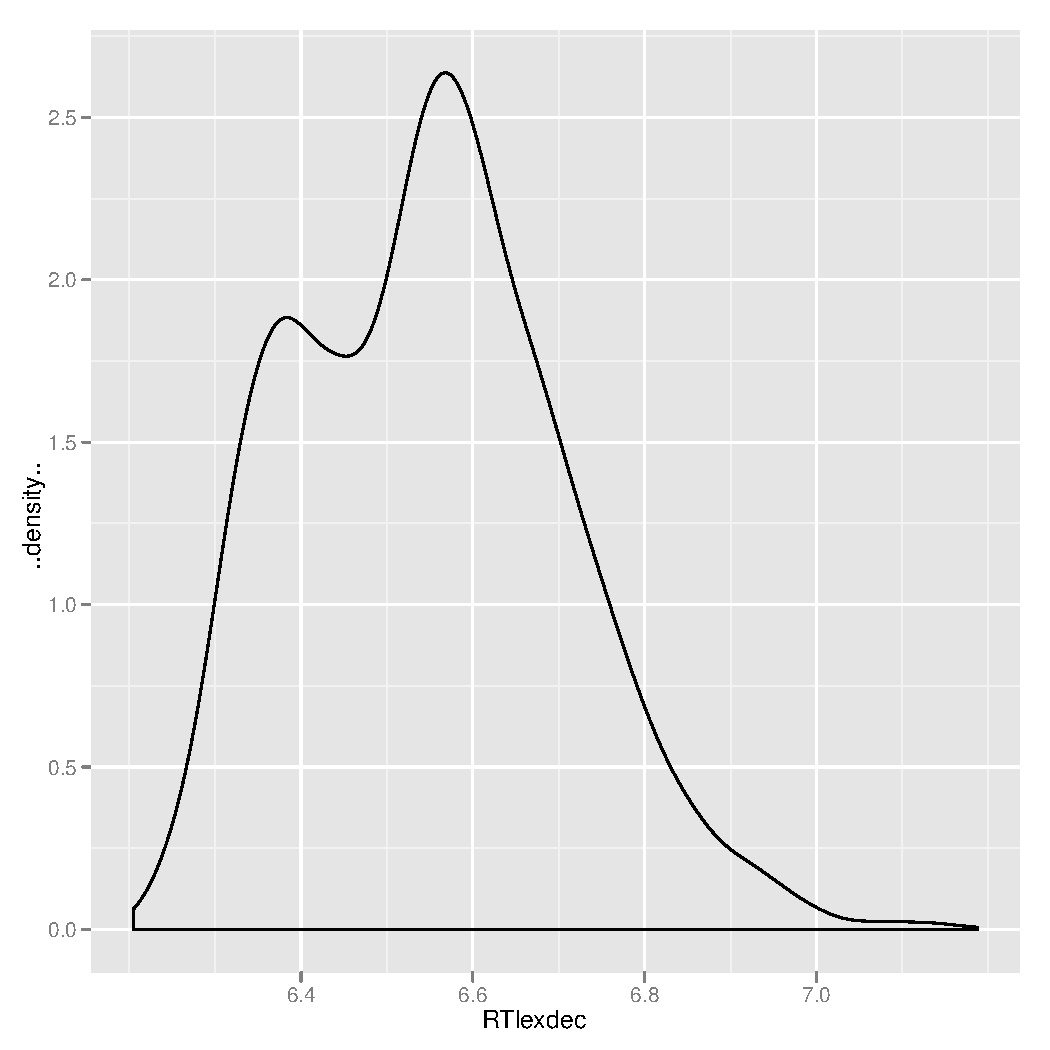
\includegraphics[width = 0.5\linewidth]{density}
  \caption{(Left) A histogram of the distribution of the \texttt{RTlexdec} response variable made with the \texttt{geom\_histogram} geom. (Right) A smooth density estimate of the same, made with the \texttt{geom\_density} geom.}
  \label{fig:one}
\end{figure}

\subsection{Plotting two dimensions}

Now we know how to plot histograms and smoothed density estimates. So far, we haven't done anything that the base R graphics system can't do. Let's move beyond base.

\newpage
\section{Beyond base}

Notice that the histogram and the density estimate seem to have two peaks. This may indicate that we are looking at two overlapping distributions. \verb!ggplot2! makes it very easy to divide data by another dimension and display it in several ways.

\subsection{Splitting by color}

First, let's try to find what predictor might be causing the two distributions. We'll consider three predictors: \verb!WordCategory!, the category of the word that is being presented, N or V; \verb!CV!, whether the word in question begins with a consonant or a vowel; and \verb!AgeSubject!, whether the subject falls into the ``young'' age group or the ``old'' age group. We'll plot a smoothed density estimate and separate the two groups based on color.

\begin{verbatim}
> p + geom_density(aes(color = WordCategory)) 
> p + geom_density(aes(color = CV))
> p + geom_density(aes(color = AgeSubject))
\end{verbatim}


\begin{figure}[htbp]
  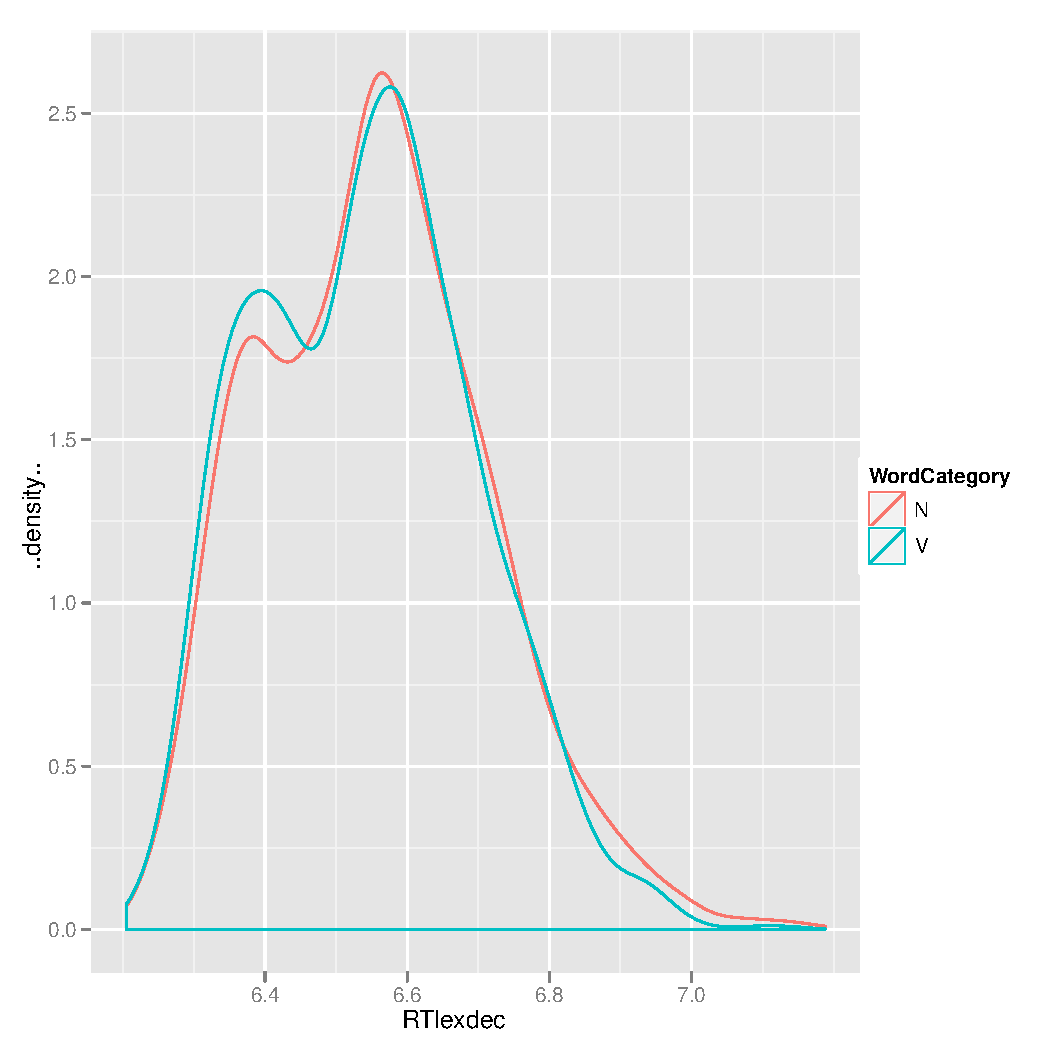
\includegraphics[width = 0.33\linewidth]{color1}%
  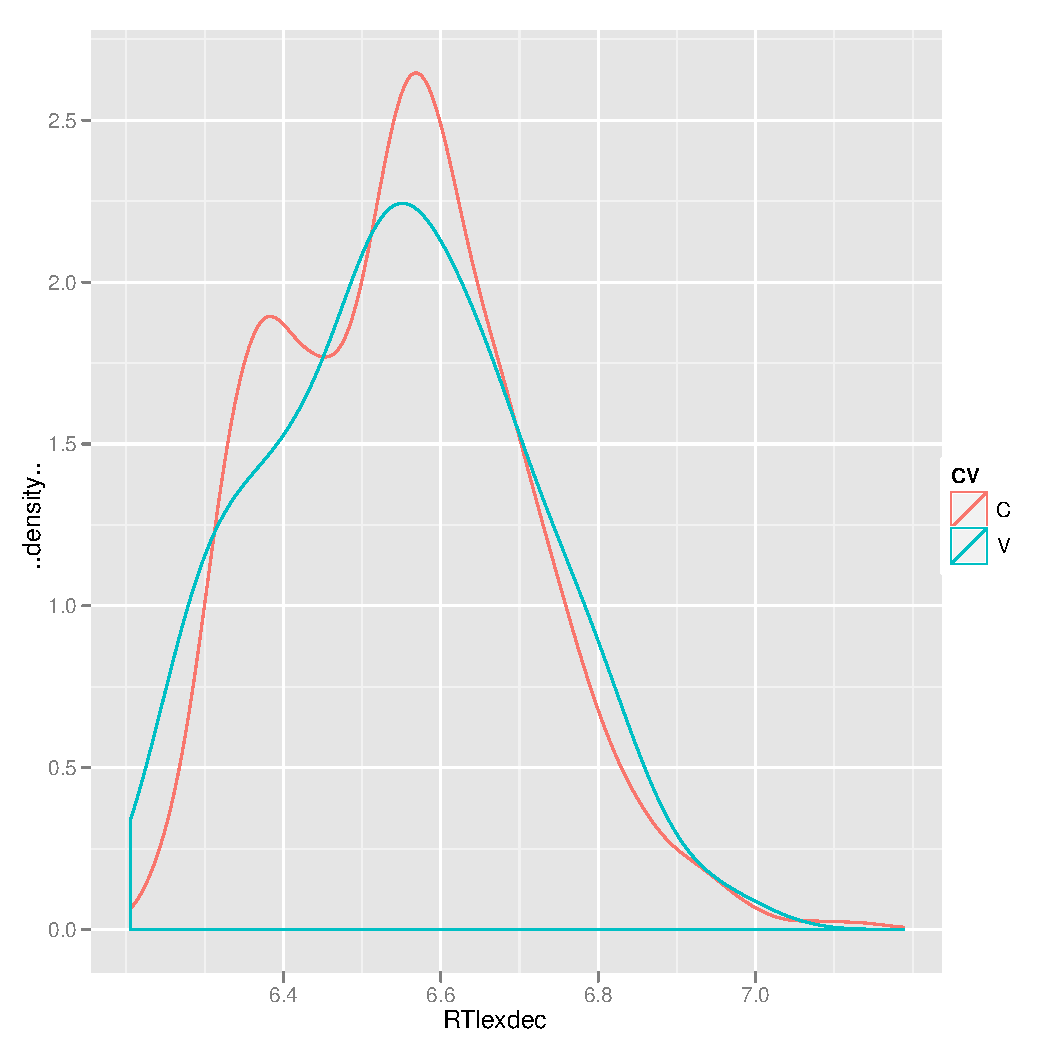
\includegraphics[width = 0.33\linewidth]{color2}
  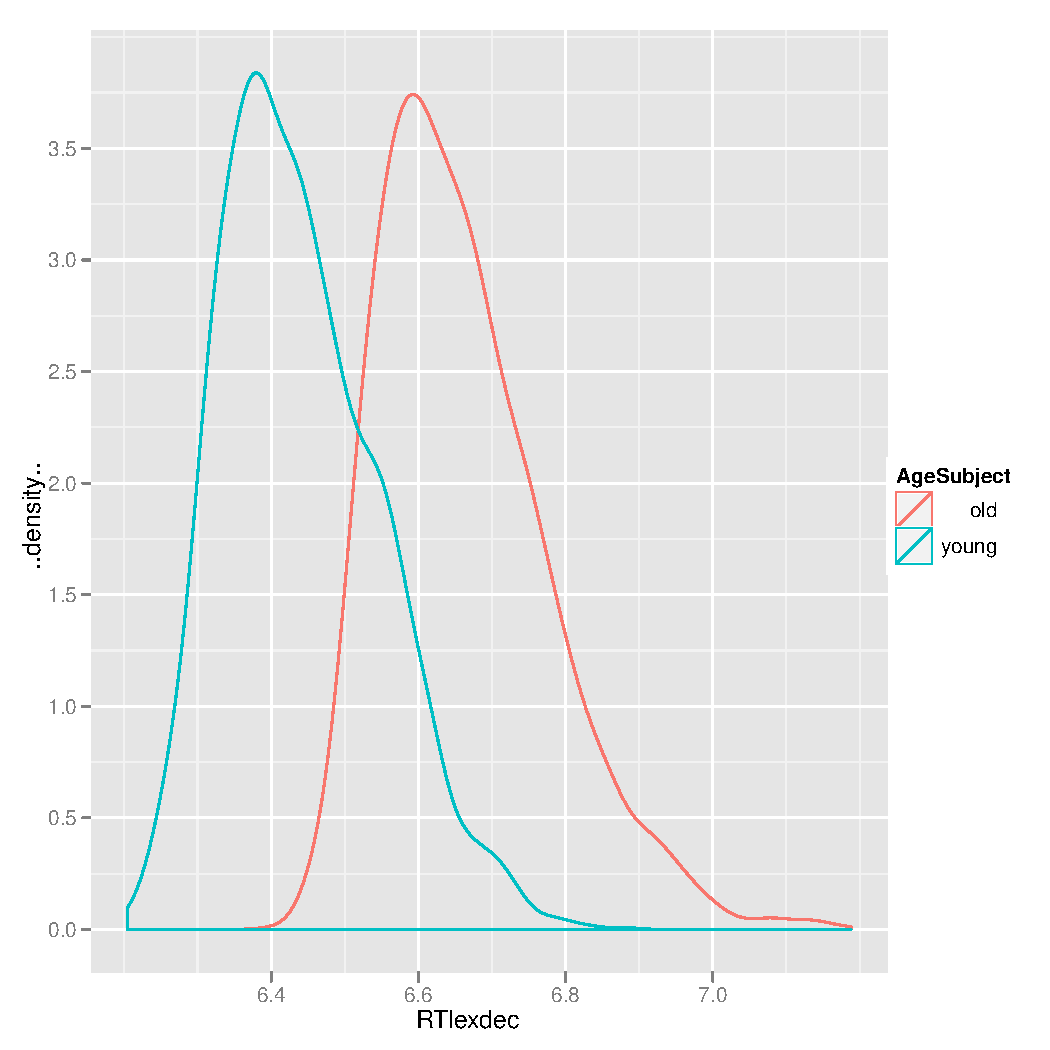
\includegraphics[width = 0.33\linewidth]{color3}%
  \caption{(Left) \texttt{WordCategory} (Center) \texttt{CV} (Right) \texttt{AgeSubject}}
  \label{fig:two}
\end{figure}

Note that the predictor you are splitting by must be a factor in R. You will get an error if you try to split by a numerical predictor. You can, however, convert integer predictors into factors with \verb!factor()!. 

\begin{verbatim}
> p + geom_density(aes(color = LengthInLetters)) # Doesn't work.
> p + geom_density(aes(color = factor(LengthInLetters))) # Does what you expect.
\end{verbatim}

\subsection{Faceting}

\begin{figure}[htbp]
  \includegraphics[width = 1\linewidth]{hexbin-facets}
  %\caption{(Left) \texttt{WordCategory} (Center) \texttt{CV} (Right) \texttt{AgeSubject}}
  \label{fig:three}
\end{figure}

  




\end{document}
